\section{Auswertung}
\label{sec:Auswertung}
Zuerst wird der Energieverlust der Alphateilchen bestimmt. Dieser wird ermittelt, 
indem die Energie der Teilchen gegen die effektive Weglänge aufgetragen wird. 
Die effektive Weglänge wird dabei mithilfe von Formel (\ref{eqn:effektive_Laenge}) berechnet. 
Die Energie wird durch einfachen Dreisatz aus den Informationen berechnet, dass
diese proportional zum Channel, indem die meisten Teilchen gemessen werden, ist und 
der Channel, indem bei einem Druck von $0 \unit{\milli\bar}$ die meisten Teilchen sind,
eine Energie von $4 \unit{\mega\electrovolt}$ hat. Die Anzahl der Teilchen, 
die abhängig vom Druck gemessen werden und die Channel, in dem die meisten Teilchen gezählt
werden, sind in Tabelle (\ref{tab:Abstand_1}) für einen Abstand der Probe von $x_{0,1}= 4,5 \, \unit{\centi\meter}$ und in Tabelle (\ref{tab:Abstand_2}) 
für einen Abstand der Probe von $x_{0,2} = 6 \, \unit{\centi\meter}$ aufgelistet. 

\begin{table}[H]
    \centering
    \caption{Eingestellter Druck, gemessene Pulsanzahl und Channel mit der höchsten Pulsrate bei einem Abstand von 4,5 cm}
    \label{tab:Abstand_1}
    \begin{tblr}{colspec={c c c}}
        \toprule
        $Druck \, \left[\unit{\milli\bar}]\right$ & $Anzahl der gemessenen Pulse$ &  $Channel der maximalen Pulszahl$ \\
        \midrule
        0   & 26225 & 1239 \\
        60  & 26012 & 1158 \\
        100 & 25800 & 1064 \\
        150 & 25502 & 999 \\
        200 & 25299 & 926 \\
        260 & 24468 & 839 \\
        300 & 24326 & 770 \\
        350 & 23974 & 720 \\
        400 & 22682 & 620 \\
        450 & 21331 & 511 \\
        500 & 15645 & 423 \\
        560 & 1433  & 415 \\
        \bottomrule
    \end{tblr}
\end{table}

\begin{table}[H]
    \centering
    \caption{Eingestellter Druck, gemessene Pulsanzahl und Channel mit der höchsten Pulsrate bei einem Abstand von 6 cm}
    \label{tab:Abstand_1}
    \begin{tblr}{colspec={c c c}}
        \toprule
        $Druck \, \left[\unit{\milli\bar}]\right$ & $Anzahl der gemessenen Pulse$ &  $Channel der maximalen Pulszahl$ \\
        \midrule
        0 & 16038 & 1171 \\
        50 & 15679 & 1109 \\
        100 & 15145 & 995 \\
        150 & 15031 & 921 \\
        200 & 14814 & 839 \\
        250 & 14313 & 775 \\
        300 & 13741 & 640 \\
        350 & 13076 & 614 \\
        400 & 6313 & 415 \\
        450 & 376 & 410 \\
        500 & 0 & 0 \\
        \bottomrule
    \end{tblr}
\end{table}

Die sich aus den Daten ergebenden Werte sind in Abbildung (\ref{})


% \begin{figure}
%   \centering
%   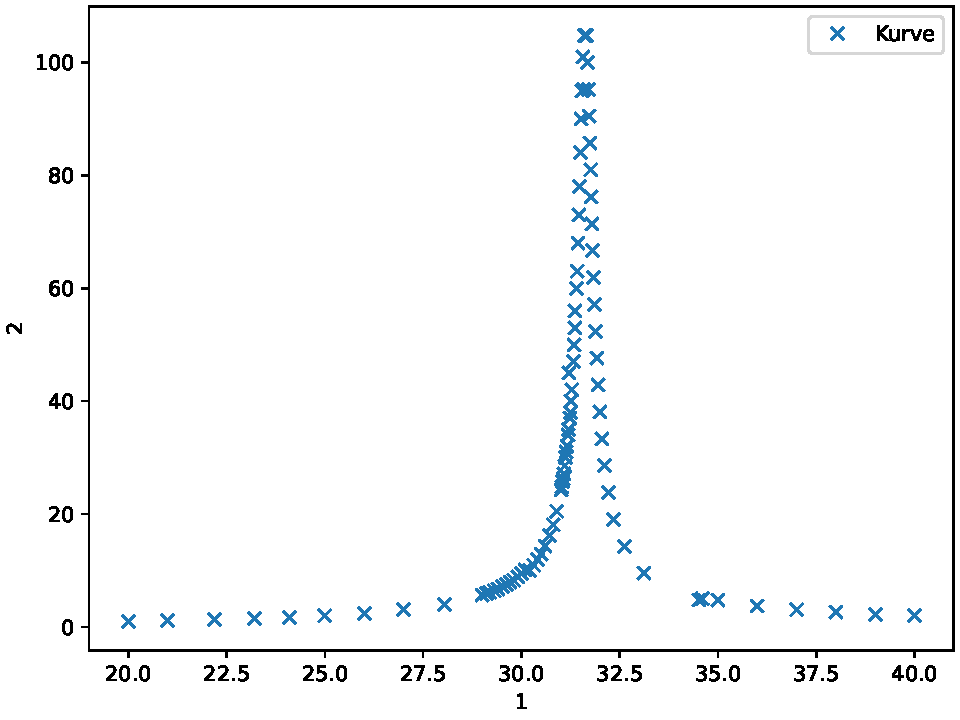
\includegraphics{plot.pdf}
%   \caption{Plot.}
%   \label{fig:plot}
% \end{figure}

%Siehe \autoref{fig:plot}!